\documentclass[letterpaper, reqno,11pt]{article}
\usepackage[margin=1.0in]{geometry}
\usepackage{color,latexsym,amsmath,amssymb,graphicx, float}
\usepackage{hyperref}

\hypersetup{
colorlinks=true,
linkcolor=magenta,
filecolor=magenta,
urlcolor=cyan,
}

\graphicspath{ {images/} }

\newcommand{\RR}{\mathbb{R}}
\newcommand{\CC}{\mathbb{C}}
\newcommand{\ZZ}{\mathbb{Z}}
\newcommand{\QQ}{\mathbb{Q}}
\newcommand{\NN}{\mathbb{N}}
\newcommand{\st}{\text{ s.t.}\ }
\newcommand{\tn}[1]{\textnormal{#1}}
\newcommand{\m}{\textnormal{ m}}
\newcommand{\s}{\textnormal{ s}}
\newcommand{\K}{\textnormal{ K}}
\newcommand{\h}{\textnormal{ h}}
\newcommand{\W}{\textnormal{ W}}
\newcommand{\J}{\textnormal{ J}}
\newcommand{\Pa}{\textnormal{ Pa}}
\newcommand{\mol}{\textnormal{ mol}}
\newcommand{\Hz}{\textnormal{ Hz}}
\newcommand{\kg}{\textnormal{ kg}}
\newcommand{\cm}{\textnormal{ cm}}
\newcommand{\mm}{\textnormal{ mm}}
\newcommand{\N}{\textnormal{ N}}

\begin{document}
\pagenumbering{arabic}
\title{PHYS 301 Homework 2}
\date{October 06, 2021}
\author{Xander Naumenko}
\maketitle

{\noindent\bf Question 1.} First calculate the divergence of the electric field: 

$$
    \nabla\cdot\vec E=\lambda\begin{bmatrix}
        \frac{\partial}{\partial x}yz\\
        \frac{\partial}{\partial y}xz\\
        \frac{\partial}{\partial z}xy
    \end{bmatrix}=\vec 0
$$

By Gauss's theorem in it's differential form, we conclude that the charge density is zero everywhere. Therefore the charge enclosed is zero. 

{\noindent\bf Question 2a.} We will choose cylindrical coordinates to integrate. By symmetry electric field will be pointed upwards in the $z$ direction. The integral is then set up as so: 

$$
    \int_S  d\vec E=\int_S \frac{k\hat r^\prime}{r^2+z^2}dq=\int_0^R\int_0^{2\pi}\frac{kz\sigma}{(r^2+z^2)^{3/2}}r  d\phi dr
$$

Letting $u=r^2+z^2$, and we get 

$$
    =-2\pi zk\sigma u^{-\frac12}\bigg|_0^R=2\pi k\sigma(1-\frac z{\sqrt{R^2+z^2}})
$$

As stated previously this is the magnitude of the electric field, oriented along the $\hat z$ direction. Taking the divergence of the electric potential we found in class we get 

$$
    \vec E=-\nabla\cdot V=-\nabla\cdot (2k\sigma\pi(\sqrt{z^2+R^2}-|z|))=2\pi k\sigma(1-\frac z{\sqrt{R^2+z^2}})
$$

These confirm each other as they lead to the same result. Note that for both of these we implicitly assume that $z>0$, for $z<0$ the sign is flipped. 

{\noindent\bf Question 2b.} For $z<<R$ the expression becomes 

$$
    E_z\approx2\pi k\sigma(1-\frac zR)\approx 2\pi k\sigma
$$

This implies that the field trends towards a constant field near the disc, which makes sense given up close it looks like an infinite sheet of charge. For $z>>R$, we can expand with a taylor expression of $\frac1{\sqrt{1+x^2}}\approx1-\frac{x^2}2$. Then we get 

$$
    E_z=2\pi k\sigma(1-\frac{z}{z\sqrt{1-\frac{R^2}{z^2}}})\approx 2\pi k\sigma(\frac{R^2}{2z^2})
$$

Thus for this case the electric field looks like that of a point charge. 

{\noindent\bf Question 3a.} On the $z$ axis, by symmetry the electric field is oriented along the $z$ axis. Then the electric field is 

$$
    \vec E= k\hat z\int_{-\infty}^0 \frac{\lambda}{(z-l)^2}dl=k\hat z\frac{\lambda}{z-l}\bigg|_{-\infty}^0=\frac{k\lambda\hat z}{z}
$$

{\noindent\bf Question 3b.} For along the $x$ axis, we can no longer make assumptions about the direction of the field. We also have that for an infinitesimal piece of charge along the line, the radial vector pointing from it to the point we're measuring at ($z=l$) is $\vec r=x\hat i-l\hat k$

$$
    \vec E=\int_{-\infty}^0|dE|\cdot \hat r=\int_{-\infty}^0\frac{kdq}{r^2}\cdot \frac{\vec r}{r}=k\int_{-\infty}^0\frac{\lambda}{(x^2+l^2)^{3/2}}\begin{bmatrix}x\\0\\-l\end{bmatrix}dl
$$

We will compute the two integrals separately. The $z$ component is easier, and we get 

$$
    E_z=\int_{-\infty}^0\frac{-\lambda k l}{(x^2+l^2)^{3/2}}dl=\lambda k\frac1{\sqrt{x^2+l^2}}\bigg|_{-\infty}^0=\frac{\lambda k}{x}
$$

For the $x$ component, let $l=x\tan\theta$. Then $dl=x\sec^2\theta d\theta$ and we get 

$$
    \int_{-\pi/2}^0\frac{\lambda kx}{x^3(\tan^2\theta + 1)^{3/2}}x\sec^2\theta d\theta=\int_{-\pi/2}^0\frac{\lambda k}x \cos\theta d\theta=\frac{\lambda k}{x}\sin\theta\bigg|_{-\pi/2}^0=\frac{\lambda k}x
$$

Thus the final field is $\vec E=\frac{\lambda k}{x}(\hat i+\hat k)$

{\noindent\bf Question 4.} First, we normalize the charge density. To do this we compute a volume integral using integration by parts twice: 

$$
    Q_{\text{total}}=\int_V \rho d\tau=\int_0^\pi\int_0^{2\pi}\int_0^\infty\rho_0e^{-2r/a_0}r^2\sin\theta drd\phi d\theta=4\pi\rho_0(-\frac{a_0r^2}2e^{-2r/a_0}+\int a_0re^{-2r/a_0}dr)
$$

$$
    =4\pi\rho_0(-\frac{a_0r^2}2e^{-2r/a_0}-\frac{a_0^2r}2e^{-2r/a_0}+\int \frac{a_0^2}2e^{-2r/a_0}dr)
$$ 
    
$$
    =-\pi\rho_0e^{-2r/a_0}(2a_0r^2+2a_0^2r+a_0^3)\bigg|_0^{\infty}
$$

Since $e^r$ asymptotically grows faster than any polynomial we evaluate this expression as 

$$
    =a_0^3\pi\rho_0=-e^-\Rightarrow \rho_0=-\frac{e^-}{a_0^3\pi}
$$

Here $e^-$ is the elementary charge. To find the electric field, note the symmetry in the situation which means the field points radially outward. Constructing a gaussian sphere with radius $r$ we can use the indefinite integral derived above to get the electric field magnitude: 

$$
    E\cdot4\pi r^2=\frac{Q_{enclosed}}{\epsilon_0}
$$

$$
    =\frac{e^-}{\epsilon_0}-\frac{e^-}{a_0^3\epsilon_0}(a_0^3-e^{-2r/a_0}(2a_0r^2+2a_0^2r+a_0^3))=\frac{e^-}{a_0^3\epsilon_0}e^{-2r/a_0}(2a_0r^2+2a_0^2r+a_0^3)
$$

$$
    \Rightarrow E=\frac{e^-}{4\pi r^2 a_0^3\epsilon_0}e^{-2r/a_0}(2a_0r^2+2a_0^2r+a_0^3)
$$

A graph of this field along with that of a proton can be seen in figure \ref{fig:q4}. 

% https://www.desmos.com/calculator/xaazvulwk5
\begin{figure}[htbp]
\centering
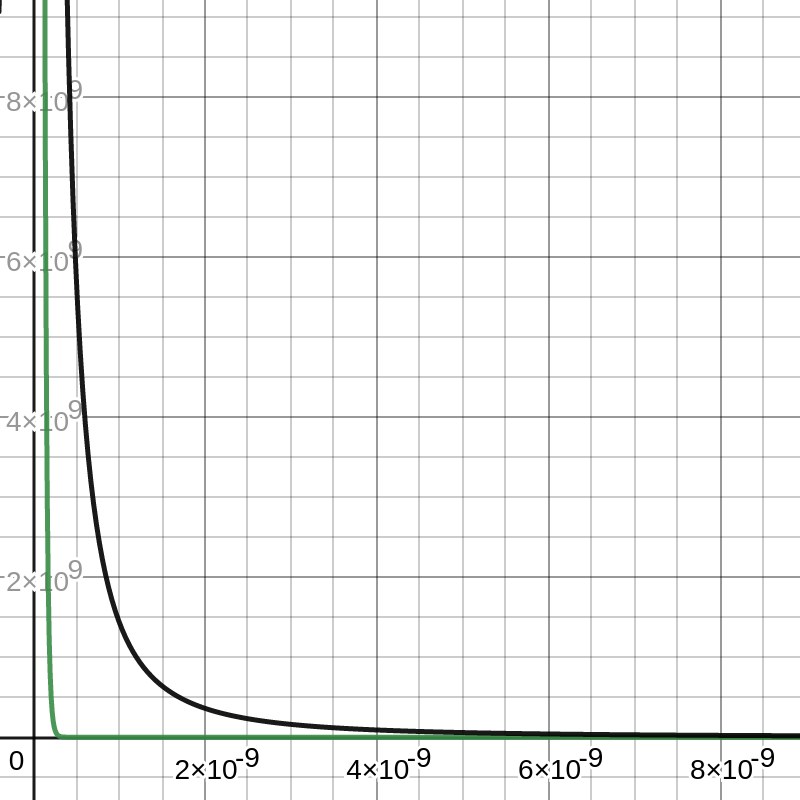
\includegraphics[width=\textwidth]{q4}
\caption{Graph of electric field of atom as a whole (green) and that of just the proton (black) as a function of distance. }
\label{fig:q4}
\end{figure}

{\noindent\bf Question 5.} We will superposition to solve the problem. First consider the sphere of charge by itself, and using Gauss's law we get that for any distance $r$ away from the distance of the big sphere, we have

$$
    E\cdot 4\pi r=\frac{Q_{enclosed}}{\epsilon_0}=\frac{\frac43\pi r^3\rho}{\epsilon_0}\Rightarrow E=\frac{\rho r}{3\epsilon_0}\Rightarrow \vec E=\frac{\rho}{3\epsilon_0}\vec r
$$

Next consider a small sphere at point $a$ constructed of negative charge of density $\rho$. The magnitude of the field produced by this sphere, again using Gauss's law is 

$$
    E\cdot 4\pi |\vec r-\vec a|=\frac{Q_{enclosed}}{\epsilon_0}=\frac{-\frac43\pi |\vec r-\vec a|^3\rho}{\epsilon_0}\Rightarrow E=\frac{-\rho |\vec r-\vec a|}{3\epsilon_0}
$$

For the direction the electric field is pointing away from $\vec a$ towards $\vec r$, so the total electric field from this smaller sphere is $\vec E=\frac{\rho}{3\epsilon_0}(\vec r-\vec a)$. Using superposition if we put these two spheres together, we arrive at the same situation as described in the original question and we find that the total electric field is 

$$
    \vec E=\frac{\rho}{3\epsilon_0}\vec r-\frac{\rho}{3\epsilon_0}(\vec r-\vec a)=\frac{\rho}{3\epsilon_0}\vec a
$$

\end{document}